\documentclass[11pt]{article}
\usepackage[T1]{fontenc}
\usepackage[utf8]{inputenc}
\usepackage{lmodern,microtype}
\usepackage[margin=1in,headheight=14pt]{geometry}
\usepackage{amsmath,amssymb,amsthm,mathtools}
\usepackage{booktabs,longtable,tabularx,array}
\usepackage{graphicx,xcolor,enumitem,fancyhdr}
\usepackage{listings,xurl}
\definecolor{ink}{RGB}{24,47,73}
\definecolor{teal}{RGB}{0,103,113}
\definecolor{light}{RGB}{243,246,249}
\usepackage[colorlinks=true,linkcolor=ink,citecolor=teal,urlcolor=teal]{hyperref}
\usepackage[nameinlink,noabbrev]{cleveref}
\hypersetup{pdftitle={Modular Boundary Responses for Unknot Recognition},
 pdfauthor={ProveIt research continuation prepared with OpenAI ChatGPT},
 pdfsubject={Exact modular Euler obstructions and singular-safe boundary compression}}
\pagestyle{fancy}
\fancyhf{}
\fancyhead[L]{\small\color{ink}Modular boundary responses}
\fancyhead[R]{\small ProveIt research notes}
\fancyfoot[C]{\thepage}
\renewcommand{\headrulewidth}{0.3pt}
\setlength{\parskip}{3pt}
\setlist{itemsep=3pt,topsep=5pt}
\emergencystretch=2em
\newcolumntype{P}[1]{>{\raggedright\arraybackslash}p{#1}}
\newtheorem{theorem}{Theorem}[section]
\newtheorem{lemma}[theorem]{Lemma}
\newtheorem{proposition}[theorem]{Proposition}
\newtheorem{corollary}[theorem]{Corollary}
\theoremstyle{definition}
\newtheorem{definition}[theorem]{Definition}
\newtheorem{example}[theorem]{Example}
\theoremstyle{remark}
\newtheorem{remark}[theorem]{Remark}
\DeclareMathOperator{\Kh}{Kh}
\DeclareMathOperator{\rank}{rank}
\DeclareMathOperator{\nullity}{nullity}
\DeclareMathOperator{\bal}{bal}
\DeclareMathOperator{\diag}{diag}
\DeclareMathOperator{\sgn}{sgn}
\newcommand{\F}{\mathbb F}
\newcommand{\Z}{\mathbb Z}
\newcommand{\Q}{\mathbb Q}
\newcommand{\Khred}{\widetilde{\Kh}}
\newcommand{\norm}[1]{\left\lVert #1\right\rVert_1}
\newcommand{\code}[1]{\texttt{\small #1}}
\newcommand{\basecommit}{\texttt{8a95834940cf77cdab1b39571ffc102ca8b6bede}}
\lstset{basicstyle=\ttfamily\small,breaklines=true,columns=fullflexible,
 keepspaces=true,showstringspaces=false,backgroundcolor=\color{light},
 frame=single,rulecolor=\color{light},xleftmargin=4pt,xrightmargin=4pt}
\title{\color{ink}\bfseries Modular Boundary Responses\\for Unknot Recognition\par
 \vspace{0.5em}\large Certified Euler obstructions, singular-safe compression,\\
 and deterministic threshold refinement}
\author{ProveIt research continuation\\
 \small Prepared for Vladimir Reshetnikov with OpenAI ChatGPT}
\date{8 October 2026}
\begin{document}
\maketitle
\thispagestyle{empty}
\begin{abstract}
We continue the implementation program in \emph{ProveIt/Topology/UnknotRecognition}.
The maintained marked-continuation observer reconstructs closed diagrams and
evaluates integer signed-Laplacian determinants. A prior research prototype
reuses a rational boundary response. We give and implement a finite-field
continuation of that prototype, retaining singular interior directions and
reusing the actual suffix geometry. Its auxiliary primes reduce integer Euler
characteristics; the underlying Khovanov complex remains over $\F_2$.

Three quantitative results organize the improvement. First, a checkerboard
suffix with $b>0$ frontier darts has exactly $b/2$ black open face fragments,
so every potentially nonzero residual determinant has dimension at most $b-2$.
Second, modular residues of whole completed components give sound, monotone
lower bounds on reduced Khovanov rank. Retaining the exact Euler sum yields a
closed formula for the strongest $\ell^1$ lower bound with those data.
Third, if each component coordinate is bounded by $C_a$, accumulated modulus
$M>\max_a C_a$ already makes the threshold-one test exact; unique coefficient
reconstruction is unnecessary. We prove explicit bounds on $C_a$ and identify
the distinction between this completion theorem and the finite prime palette
implemented by the prototype.

Fresh-setup paired measurements show a $26.67$-fold improvement over the
maintained direct evaluator and a $3.97$-fold improvement over the earlier
rational prototype on a 200-query workload with 47 genuine interior vertices.
The small-interior cases and all seven raw recognition examples show regressions.
The new backend therefore remains optional. No general quasi-polynomial
running-time bound for the maintained recognizer is proved. The package
includes proofs, source changes, independent arithmetic and geometric audits,
replay checks, full timing samples, and a targeted research agenda.
\end{abstract}
\vfill
\noindent\small\textbf{Research status.} This is an AI-assisted working paper, cross-checked with separate
arithmetic routines and exact small-instance computations, not a refereed publication. Established results,
repository-derived constructions, proved refinements, experiments, and open
obligations are distinguished throughout. The source baseline is recorded
exactly in the accompanying provenance file.
\newpage
{\small\setlength{\parskip}{0pt}\tableofcontents}
\newpage
\section{Scope, source audit, and principal conclusions}
\label{sec:context}

\subsection{The question addressed}

The practical question is whether repeated observations of a partially computed
knot complex can become sufficiently cheap to justify earlier recognition.
The asymptotic question is whether such observations can help the program avoid
the exponentially large intermediate representations that obstruct a general
quasi-polynomial bound. These questions require different evidence. A fast
determinant subroutine answers the first only on workloads where it is used
often enough. It answers the second only when accompanied by control of the
number and size of the complexes that must be constructed before it succeeds.

The source examined here is the public ProveIt revision
\begin{center}\basecommit.\end{center}
All references to the ``maintained'' implementation mean that pinned revision,
before this package's additions. The repository already contains 28 numbered
reports, numerous integrated improvements, and a Python implementation far
beyond the earliest scanning baseline. Its relevant files are
\path{fast/fastunknot/shadow_scan.py},
\path{fast/fastunknot/integer_determinant.py},
\path{fast/fastunknot/tait_blocks.py}, and the research prototype
\path{fast/determinant_research/boundary_tait.py}.
The maintained explanations are
\path{synthesis/determinant_continuations.tex},
\path{synthesis/boundary_reuse.tex},
\path{synthesis/tait_blocks.tex}, and
\path{synthesis/shadow_fallback.tex} \cite{proveit}.

Report 26 already supplies the marked four-residue obstruction and a
singular-safe rational terminal kernel. Later maintained work supplies cut-face
fragments, a boundary-only geometric acceptance check, articulation factorization
of direct cofactors, and a budgeted Euler fallback. We use those results openly.
Reintroducing a Schur complement or an Euler norm without this attribution would
misstate the continuation's contribution.

\subsection{What this continuation adds}

The deliverable has four connected parts.

\begin{enumerate}
\item An exact terminal count, $t=b/2$, and the resulting $b-2$ residual
dimension bound for a nonempty frontier. This sharpens the earlier loose linear
bound for the actual cut-face construction.
\item A modular observer with a fully proved integer interpretation. It combines
congruences by the Chinese remainder theorem (CRT), retains the exact coordinate
sum, and solves a four-dimensional integer norm minimization explicitly.
\item A deterministic threshold completion theorem. The modulus required to
decide whether the existing bound exceeds one is smaller than the modulus
required to reconstruct all its integer coordinates.
\item An optional implementation in the maintained package, with independent replay of its
positive observations and paired comparisons against both relevant predecessors.
\end{enumerate}

The basic modular-determinant idea is established numerical algebra
\cite{dumasurbanska}. Boundary response matrices also have a substantial
literature \cite{kenyonwilson}. Our claims concern the explicit proofs and
implementation given here; a limited literature search is not a certification
of historical priority for every elementary lemma.

\begin{samepage}
\begin{theorem}[Combined observer guarantee]
\label{thm:main}
Suppose a validated classical knot diagram has a proper scan prefix whose
relative complex has been obtained by the algebraically valid operations
implemented by the maintained scanner. Let $\mathcal C_a$ be its whole differential components, with positive
multiplicities $m_a$, and let $x_a\in\Z^4$ be the marked completed Euler vectors.
For a product $M$ of distinct validated odd primes, the algorithm below computes
a number $L_M$ satisfying
\[
 0\le L_M\le B_4:=\sum_a m_a\norm{x_a}
 \le \dim_{\F_2}\Khred(K;\F_2).
\]
It may therefore return \code{KNOTTED} whenever $L_M>1$.
If $|x_{a,r}|\le C_a$ and $M>\max_a C_a$, then
\[
             L_M>1\quad\Longleftrightarrow\quad B_4>1.
\]
For a suffix with $b>0$ frontier darts, each modular determinant query after
preparation uses a matrix of dimension at most $b-2$, or returns the proved
zero residue without forming that matrix. These statements remain valid at
primes where the interior matrix becomes more singular.
\end{theorem}
\end{samepage}

The proof is distributed through \cref{sec:euler,sec:geometry,sec:modular}.
The hypothesis about the relative complex is essential: a randomly chosen
matrix satisfying $d^2=0$ is not enough. Likewise, $L_M\le1$ is not an unknot
certificate, even when the threshold comparison with $B_4$ is complete.

\subsection{Current literature and the complexity target}

Lackenby's July 2026 preprint develops an explicit hierarchy framework and
efficiently encoded certificates \cite{lackenby2026}. Proposition 9.1 bounds
the number of iterations by
\[
                         L(g+1)^L,
\]
where $L$ is a hierarchy-length bound and $g$ a pattern-complexity bound.
The refined algorithm controls hierarchy length using handle complexity;
Theorem 14.1 establishes, under its manifold and handle-structure
hypotheses, the existence of an essential hierarchy with a polynomial-size
encoding and polynomial-time verification. The paper leaves the proposed speed-up to further work. These are
substantial algorithmic foundations, but polynomial certificate verification
does not supply a polynomial or quasi-polynomial certificate-construction time.

The exact exponent also deserves care. The March 2021 Oxford technical
handout states $2^{O((\log N)^3)}=N^{O((\log N)^2)}$ \cite{lackenbytalk}.
The Oxford seminar abstract instead states $N^{O(\log N)}$
\cite{lackenbyabstract}. Both are
quasi-polynomial, but the latter is stronger. We keep the repository's stronger
target visible while using $2^{(\log N)^{O(1)}}$ when discussing the broad class.
No result here converts one announced exponent into another.

A separate September 2026 preprint by Musick explicitly claims polynomial
unknot recognition \cite{musick}. This changes what a current literature note
must acknowledge. The present work does not validate or integrate that claimed
algorithm. A limited review identifies the grammar-to-geometric-local-minimum
step and total compressed-description accounting as obligations for a separate
audit; it supplies no counterexample or disproof. Our definite complexity claim
is about the maintained ProveIt implementation: it still has no established
general quasi-polynomial guarantee.

The representation obstacle is concrete. In their January 2026 preprint,
Kelom\"aki and Sch\"utz prove
exponential behavior for basis-oriented scanning and divide-and-conquer on
particular positive or alternating three-braids, while also obtaining
polynomial-time structural formulas for three-braid Khovanov homology
\cite{kelomaki}. Thus a small frontier and a large explicit homology basis can
coexist. A succinct answer may nevertheless be tractable. This continuation
compresses an observation of the complex; it does not prove that the complex
itself remains succinct.

\subsection{Reading the empirical conclusion}

On the favorable repeated-query workload, 47 interior vertices are eliminated
once and 200 actual boundary matchings are observed. The modular path is
$26.67$ times faster than the maintained direct path and $3.97$ times faster
than the rational prototype. At 127 interior vertices and 50 queries, the
corresponding ratios are $10.74$ and $10.22$.

Conversely, the all-terminal workload slows down, the smallest nontrivial
interior favors the rational prototype, and the raw recognizer examples all
favor the existing direct observer. These measurements justify an optional
backend and further scheduling research. They do not justify changing the
default recognizer or claiming a general recognition speed-up.

\begin{center}
\begin{tabularx}{\textwidth}{@{}P{0.28\textwidth}X@{}}
\toprule
Claim category & Status in this package\\
\midrule
Modular arithmetic soundness & Proved, implemented, independently audited.\\
Exact terminal count & Proved for the checked cut-face representation.\\
Deterministic threshold completion & Proved; implementation reports whether its finite palette suffices.\\
Repeated-query acceleration & Measured with setup included and both predecessors compared.\\
Whole-recognizer acceleration & Not demonstrated on the tested corpus.\\
General quasi-polynomial recognition & Not established by this work.\\
\bottomrule
\end{tabularx}
\end{center}

\section{Marked completion and the integer Euler obstruction}
\label{sec:euler}

\subsection{Relative complexes and a persistent marked point}

Fix a classical one-component planar diagram $D$ with $N$ crossings and a
validated permutation of its crossings. A proper prefix leaves a suffix with
$n\ge1$ crossings. The scanning construction represents the prefix by a complex
in the dotted cobordism category. Each object is a boundary matching with its
homological and quantum shifts; closed circles have been removed through the
standard delooping operations. Differentials, cancellations, and their homotopies
are the actual maps supplied by this construction \cite{barnatan2005,barnatan2007}.

Choose a point on an edge incident to the final unprocessed crossing. It remains
in the suffix at every proper-prefix observation. On completion, the marked
circle carries the action of $A=\F_2[x]/(x^2)$. The marked quotient is applied
after the actual suffix has been attached.

\begin{lemma}[Why completion and reduction preserve the contractions]
\label{lem:marked}
Suppose the prefix complex is decomposed and simplified by chain maps and
chain homotopies that commute with the marked action after completion. Applying
the marked quotient preserves every recorded chain-homotopy equivalence.
\end{lemma}
\begin{proof}
If maps $f,g$ and a homotopy $h$ satisfy $fg-1=dh+hd$, all maps are
$A$-linear. Their induced maps on the quotient satisfy the same equality,
because passage to the quotient respects composition and addition. The other
homotopy identity is treated identically. This argument does not require the
quotient functor to be flat or exact on arbitrary short exact sequences.
\end{proof}

Let $\mathcal C_a$ be a whole connected component of the differential graph after such
simplification. The absence of differentials between these groups gives a
direct sum of complexes. Completing with the actual suffix and applying the
marked quotient gives
\begin{equation}
 \Khred(K;\F_2)\cong
 \bigoplus_a H\!\left(\widetilde{\operatorname{cl}}(\mathcal C_a)\right)^{\oplus m_a},
 \label{eq:completed-sum}
\end{equation}
up to recorded shifts, whose effect on the norms below is harmless. Shared
copies can have different global shifts; each has the same norm.

\subsection{Four integer coordinates}

For a finite bigraded complex $X$, define its residue-four Euler vector by
\begin{equation}
 \sigma_r(X)=\sum_{h,\ j\equiv r\pmod4}(-1)^h\dim_{\F_2}X^{h,j},
 \qquad 0\le r<4.
 \label{eq:sigma}
\end{equation}
Differentials preserve the quantum grading, so taking Euler characteristics
after homology leaves this vector unchanged. A homological shift negates all
four coordinates when the shift is odd. A quantum shift cyclically permutes
them. Both preserve the $\ell^1$ norm.

\begin{proposition}[Existing marked-component bound]
\label{prop:B4}
With the provenance of \cref{lem:marked}, put
$x_a=\sigma(\widetilde{\operatorname{cl}}(\mathcal C_a))$. Then
\[
 B_4=\sum_a m_a\norm{x_a}
 \le\dim_{\F_2}\Khred(K;\F_2).
\]
In particular, $B_4>1$ certifies that $K$ is nontrivial.
\end{proposition}
\begin{proof}
For each residue, let $e_r,o_r$ be the total dimensions of the even and odd
homology groups. Then $|e_r-o_r|\le e_r+o_r$. Summing over residues and
using \cref{eq:completed-sum} proves the inequality. Reduced Khovanov rank one
detects the unknot; the maintained $\F_2$ criterion follows from the standard
unknot-detection theorem and change-of-coefficients implications
\cite{kronheim}. The rank-one implication is the existing recognition premise,
not a new assertion about the auxiliary prime fields used below.
\end{proof}

\paragraph{The order of operations is part of the theorem.}
For each whole component, sum all signed, shifted object vectors first. Then
take a norm, and finally sum with positive multiplicities. A pair of object
vectors $u$ and $-u$ may belong to one contractible complex. Their true Euler
contribution is zero, while $\norm{u}+\norm{-u}$ is positive. Neither modular
arithmetic nor early stopping permits taking a norm midway through this sum.
Stopping after a \emph{completed} component is safe because all remaining
component norms are nonnegative.

\subsection{Recovering the vector from two scalar evaluations}

We use the repository's raw reduced polynomial convention
\begin{equation}
 J_D(q)=\sum_{s\in\{0,1\}^n}(-q)^{|s|}
                 (q+q^{-1})^{c(s)-1}.
 \label{eq:raw-J}
\end{equation}
Here $c(s)$ counts the circles of the smoothing. The completion contains no
explicit crossing-free circles outside this diagram; previously delooped
circles are represented by the prefix's shifted objects and multiplicities.

Changing a smoothing changes the circle count by one in parity. Hence all
quantum degrees in \cref{eq:raw-J} have parity
$\epsilon=(c(0)-1)\bmod2$. If
\[
 a=J_D(1),\qquad d=i^{-\epsilon}J_D(i)\in\Z,
\]
the only potentially nonzero coordinates are
\begin{equation}
 \sigma_\epsilon=\frac{a+d}{2},\qquad
 \sigma_{\epsilon+2}=\frac{a-d}{2}.
 \label{eq:two-values}
\end{equation}
Indeed, evaluation at one adds the two residue sums, while evaluation at $i$
subtracts them after removing the common factor $i^\epsilon$. In particular,
\begin{equation}
                     \norm{\sigma(D)}=\max(|a|,|d|).
 \label{eq:maxnorm}
\end{equation}
This identity will give small and explicit coefficient bounds.

\subsection{The exact evaluation at one}

Let $c$ be the number of link components and $c_0=c(0)$ the all-zero circle
count. In the raw convention,
\begin{equation}
                  a=(-1)^{n+c+c_0}2^{c-1}.
 \label{eq:euler-sign}
\end{equation}
One way to see the sign is to choose an orientation and write $h$ for the
number of one-smoothings in its Seifert state and $s$ for its Seifert circles.
Circle parity gives $s\equiv c_0+h\pmod2$. The orientable Seifert surface
has $s-n\equiv c\pmod2$. Thus $h\equiv n+c+c_0\pmod2$.
The normalized reduced evaluation at one is $2^{c-1}$, and the raw shift
supplies the sign above.

The existing implementation computes the same integer by independently
orienting the completed link. A reusable boundary connectivity summary can
instead determine $c$ and $c_0$ without revisiting the suffix. Both versions
remain available as cross-checks. The integer $2^{c-1}$ has $O(n)$ bits; a
boundary-sized combinatorial traversal is not automatically a boundary-only
bit-cost bound for constructing this integer.

\subsection{The signed determinant and its phase}

For a connected completed projection, checkerboard color its regions. At a
crossing $e$, let $b_e$ be the smoothing bit that does not join its black
sectors, and put $w_e=(-1)^{b_e}$. Set $B=\sum_e b_e$. If $G$ is the signed
black Tait graph with $v$ vertices, then
\begin{equation}
 J_D(i)=(-i)^{B+v-1}\tau(G),\qquad
 \tau(G)=\det L_G^{(0)},
 \label{eq:tait}
\end{equation}
where $L_G^{(0)}$ is a grounded Laplacian cofactor.

At $q=i$, all states except one-circle states vanish. Those states correspond
to spanning trees of the Tait graph. Their phases give \cref{eq:tait}; the
matrix-tree expansion is polynomial in the edge weights, so the signs do not
require a positive Laplacian. Loops contribute to $B$, although their incidence
vectors vanish in the Laplacian. Removing them from the phase would invalidate
the observation. If the projection is disconnected, every smoothing has more
than one circle and $J_D(i)=0$.

For connected accepted geometry we also have
\[
                       B+v-1\equiv\epsilon\pmod2.
\]
Choose any unsigned spanning tree. Its one-circle state has smoothing-weight
parity $B+v-1$, while circle parity gives $|s|\equiv c_0-1\pmod2$.
This proves the identity even when the signed tree sum cancels.
It is a combinatorial parity condition, not merely a check that the computed
Gaussian integer lies on the correct axis. The implementation checks it even
when a modular determinant vanishes, so a zero residue cannot conceal a phase
inconsistency.

\subsection{Relative shifts and multiplicity saturation}

The maintained grading recovery assigns a relative quantum shift $t_o$ to
every object in a component, checking every nonzero differential and cycle.
For a map of dot degree $d$ between matchings with $m$ arcs and $c$ glued
circles, its equation is $t_{\rm target}-t_{\rm source}=m-c+2d$.
Object $o$ contributes $(-1)^{h_o}\operatorname{rot}_{t_o}\sigma(D_o)$.
Only the shift modulo four is needed after consistency has been verified.

For threshold $T$, replacing a positive multiplicity $m$ by
$\min(m,T+1)$ preserves whether $m\norm{x}>T$, because the norm is an integer.
The same statement extends to sums of nonnegative terms. The maintained
scanner uses cap three; this remains sound for our threshold one. It does not
permit saturating signed Euler coefficients before aggregation.

Finally, a proper-prefix restriction remains mandatory. At the closed terminal
stage, separate unmarked scalar generators are not automatically free marked
$A$-summands. The modular observer refuses that stage. An \code{UNKNOT} verdict
comes only from the completed rank-two unreduced calculation.

\section{The exact boundary size and the modular response kernel}
\label{sec:geometry}

\subsection{Cut-face fragments}

At a suffix stage, retain its $4n$ crossing darts. Let $\rho$ rotate each
crossing counterclockwise and let $\alpha$ pair darts joined by retained
internal edges. Boundary darts are the $b$ darts where this partial involution
is undefined. The partial face map is
\[
                           f(d)=\rho(\alpha(d)).
\]
It is an injective partial map. Its components are directed cycles and directed
paths, including paths consisting of one dart. They are the closed face
fragments and open face fragments of the suffix.

A checkerboard coloring of the original diagram assigns a color to each dart
corner. Internal face-map steps preserve color. Rotating to the next corner
changes color. Therefore each fragment has one well-defined inherited color.
The common Tait graph has black fragments as vertices and one signed edge for
each retained crossing. Open black fragments are its terminals; closed black
fragments are its interior vertices. Keeping fragments is necessary: removing
the prefix may split an original region, so merely remembering its original
region identifier would not encode every completion correctly.

If boundary labels $a,b$ are paired, with darts $d_a,d_b$, the two newly inserted
face connections are
\begin{equation}
           d_a\longrightarrow\rho(d_b),\qquad
           d_b\longrightarrow\rho(d_a).
 \label{eq:face-glue}
\end{equation}
Thus completion only identifies open fragments. Closed fragments remain
distinct. These are exactly terminal identifications of the common graph.

\subsection{A precise count instead of a loose linear estimate}

\begin{theorem}[Half the frontier is the terminal set]
\label{thm:half-boundary}
For $b>0$, a checkerboard-colored suffix has exactly $b$ open face fragments,
of which exactly $b/2$ are black and $b/2$ are white. In particular, the common
Tait graph has exactly
\[
                              t=b/2
\]
terminals, whichever shading is chosen.
\end{theorem}
\begin{proof}
There are $b$ missing outgoing ends of $f$, precisely the boundary darts $d$.
There are $b$ missing incoming ends, precisely the darts $\rho(d)$ for those
same boundary darts. Every noncycle component of an injective partial map on
a finite set is a directed path with one missing incoming end and one missing
outgoing end. Hence the number of paths is exactly $b$.

Let $O_B,I_B$ denote the black missing-outgoing and missing-incoming counts,
and define $O_W,I_W$ similarly. Each path is monochromatic, giving
$O_B=I_B$ and $O_W=I_W$. Rotation changes color, so the correspondence
$d\mapsto\rho(d)$ gives $I_B=O_W$ and $I_W=O_B$. All four quantities are
therefore $b/2$. The black paths are exactly the black open fragments.
An isolated dart is a length-zero path and has the same one-incoming,
one-outgoing deficiency; it causes no exception.
\end{proof}

The earlier boundary-reuse account only required a safe $O(b)$ terminal bound.
The exact equality gives a sharper storage contract and, after elimination,
a useful explicit matrix-size bound. It does not require the entire frontier
to lie on one disk boundary, and it makes no Catalan-state assumption.

When $b=0$, there are no open fragments. The code chooses one black vertex
as an artificial grounding terminal. This case has $t=1$ and must not be
substituted into a formula involving $b-2$.

\subsection{Boundary-only geometric acceptance}

The common graph is valid for a query only after three checks.
First, the matching must cover every boundary label exactly once.
Second, every connection in \cref{eq:face-glue} must preserve the inherited
color. Third, the completed rotation system must be spherical.

Let $F$ be the number of completed faces and $k$ the number of completed
projection components. Store the numbers of closed fragments and closed
projection components during preparation. The query uses disjoint-set unions
only among open fragments and among projection components touching the
boundary. It then checks
\begin{equation}
                              F=n+2k.
 \label{eq:spherecheck}
\end{equation}
The completed ribbon graph has $V=n$, $E=2n$. Its total Euler characteristic
is $F-n=2k-2\sum_i g_i$, where $g_i\ge0$ are its orientable genera. Thus
\cref{eq:spherecheck} is equivalent to every component having genus zero.
There is no need to reconstruct all suffix faces for each query.

Both local pairings used by the Euler observer, namely opposite crossing
darts for link strands and adjacent darts for the zero smoothing, also admit
path summaries. Gluing either summary to the query matching computes $c$ and
$c_0$ in boundary-sized work. The acceptance check and these two counts together
give the exact phase and the exact value at one.

An inherited-color incompatibility declines this representation; it does not
prove knottedness. A malformed or nonspherical query is rejected as invalid
input to this oracle. In the public recognition pipeline all queried matchings
come from a validated classical scan, and a declined optional representation
causes fallback.

\subsection{The signed Laplacian quotient}

For an edge $e=uv$ with integer weight $w_e$, add
$w_e(e_u-e_v)(e_u-e_v)^{\mathsf T}$ to the Laplacian. This definition includes
parallel edges and gives zero for a loop. It yields an integer symmetric matrix
with zero row sums, without a positivity assumption.

Order the interior and terminal vertices to write
\[
               L=\begin{pmatrix} A&B\\B^{\mathsf T}&D\end{pmatrix}.
\]
For a terminal partition with $q+1$ blocks, ground its first block. Let $Q$
be the $t\times q$ matrix indicating the other blocks. Grounding the quotient
graph gives the matrix
\begin{equation}
 L_Q=\begin{pmatrix}
 A&BQ\\Q^{\mathsf T}B^{\mathsf T}&Q^{\mathsf T}DQ
 \end{pmatrix}.
 \label{eq:quotient}
\end{equation}
Every interior vertex remains separate. All terminal identifications are
encoded by the columns of $Q$. This identity follows by applying the
identification map to each edge incidence vector, so it remains valid if some
edges become loops or cancel by opposite weights.

\subsection{Elimination over each prime separately}

Fix an odd prime $p$. We reduce the original integer $L$ modulo $p$ and eliminate
only interior coordinates by symmetric pivots. If the remaining interior block
has a nonzero diagonal entry, use a one-coordinate pivot. If all its diagonals
vanish but an off-diagonal entry $u$ is nonzero, use
\[
                  P=\begin{pmatrix}0&u\\u&0\end{pmatrix},
                  \qquad \det P=-u^2\ne0.
\]
If neither exists, the remaining interior block is zero. Symmetry ensures that
these cases exhaust the possibilities.

For an invertible pivot block $P$, replace the remaining block by its Schur
complement and multiply an accumulated factor $\delta$ by $\det P$. Apply the
same operations to interior-terminal couplings and terminal-terminal entries.
Simultaneous row and column permutations contribute the square of a sign,
so they do not change the determinant. No rational pivot profile is reused
at another prime.

\begin{theorem}[Singular-safe modular response]
\label{thm:response}
Let $r=\nullity_{\F_p}A$. The preparation produces $\delta\in\F_p^\times$,
$R\in\F_p^{r\times t}$, and a symmetric $S\in\F_p^{t\times t}$ such that
for every terminal partition,
\begin{equation}
 \det L_Q=\delta\det
 \begin{pmatrix}
       0_r&RQ\\Q^{\mathsf T}R^{\mathsf T}&Q^{\mathsf T}SQ
 \end{pmatrix}
 \quad\text{in }\F_p.
 \label{eq:response}
\end{equation}
If $r>q$, the answer is zero. If $r\le q$, the residual dimension is at most
$2(t-1)$. In particular, for $b>0$ it is at most $b-2$.
\end{theorem}
\begin{proof}
At each pivot the block determinant identity proves the equality between the
old determinant and the pivot determinant times the new Schur-complement
determinant. Because only interior coordinates are eliminated, these identities
commute with multiplication of the coupling and terminal blocks by $Q$ and
$Q^{\mathsf T}$. Induction over all pivots yields \cref{eq:response}.
The remaining interior block is zero and has dimension $\nullity A$ because
every extracted pivot is nonsingular.

If $r>q$, the linear map $RQ$ has a nonzero left null vector. Extending that
vector by zeros on the terminal coordinates gives a null vector of the
residual symmetric matrix. Otherwise its dimension is $r+q\le2q\le2(t-1)$.
Apply \cref{thm:half-boundary} for the last assertion.
\end{proof}

When $r=q$, a useful independent identity is
\begin{equation}
                       \det L_Q=(-1)^r\delta\det(RQ)^2.
 \label{eq:critical}
\end{equation}
It follows by swapping the two block column groups and obtaining a block
triangular matrix. Its determinant is independent of $S$. This is a field
identity; an ordering or real sign must not be assigned to its modular value.

\begin{example}[A singular modular interior with a nonzero answer]
Take a triangle whose edge weights are $1,2,1$, and designate two vertices
as terminals. With the remaining vertex first,
\[
 L=\begin{pmatrix}
 3&-1&-2\\-1&2&-1\\-2&-1&3
 \end{pmatrix},\qquad \tau(G)=5.
\]
Over $\Q$, the interior block $[3]$ is invertible. Over $\F_3$ it is zero,
so a rational Schur complement cannot simply be reduced using its denominator.
The modular response retains one radical direction; for the unmerged terminal
partition its residual matrix has off-diagonal entry $1$ and determinant
$-1\equiv2\pmod3$, exactly $5\bmod3$.
At $p=5$, the final determinant is zero modulo five although the integer
determinant is nonzero. Neither phenomenon is an error or a reason to infer
an integer zero.
\end{example}

\subsection{What is retained and what is rebuilt}

The implementation keeps one active suffix geometry. For each requested prime
it builds one response, then caches cofactors by canonical terminal partition.
Two different boundary matchings with the same black partition share a
determinant. They still undergo their own geometry checks and may have different
link counts; these data are not inferred from the partition alone.

If $r>t-1$, every query residue is zero and the kernel can discard its unused
large residual arrays. Otherwise it retains at most an $r\times t$ coupling
and a $t\times t$ response, with $r\le t-1$. Changing the suffix discards these
active matrices. The separately cached completed values remain exact for their
full keys, which include the stage, matching, and prime.

Preparation is dense and still costs $O(v^3)$ field operations for a common
graph with $v$ vertices. The gain is that this cost is paid once per prime and
suffix, while subsequent determinants are boundary-sized. The theorem does not
guarantee that a scan asks enough queries to repay this setup.

\section{Modular lower bounds and deterministic threshold completion}
\label{sec:modular}

\subsection{A residue is information about an integer}

The complex remains over $\F_2$. Its graded dimensions and Euler sums are
integers. We use an auxiliary prime $p$ only to compute those integers modulo
$p$, evaluating \cref{eq:two-values} with $2^{-1}\in\F_p$. The Gaussian phase
is represented by one of $(1,0),(0,-1),(-1,0),(0,1)$; there is no need to adjoin
a square root of minus one to $\F_p$.

For a whole component, add the shifted object residues with their homological
signs modulo $p$. Applying CRT to this final four-vector reconstructs its
congruence class modulo the product of the processed primes. This ordering
requires only four accumulated integers per component. Reconstructing every
object's full integer determinant first is unnecessary.

\begin{samepage}
\begin{definition}[Balanced and sum-constrained norms]
For odd $M\ge3$, let $\bal_M(z)$ be the unique representative of $z\bmod M$
in $[-(M-1)/2,(M-1)/2]$. For a residue vector $z\in(\Z/M\Z)^d$, set
\[
 D_M(z)=\sum_j|\bal_M(z_j)|.
\]
If an exact integer sum $a$ is known and $a\equiv\sum_jz_j\pmod M$, set
\[
 F_M(z,a)=\min\left\{\norm{y}:y\in\Z^d,\ y\equiv z\pmod M,
                                  \sum_j y_j=a\right\}.
\]
\end{definition}
\end{samepage}

For our application, $d=4$ and $a_a=\sum_r x_{a,r}$ is the exact completed
component Euler value, obtained from the already available evaluations at one.
The two modular bounds are
\begin{equation}
 B_M=\sum_a m_aD_M(x_a),\qquad
 L_M=\sum_a m_aF_M(x_a,a_a).
 \label{eq:modular-bounds}
\end{equation}

\begin{proposition}[Soundness and monotone refinement]
\label{prop:monotone}
For every odd $M$,
\[
                 B_M\le L_M\le B_4.
\]
If $M\mid M'$, then $B_M\le B_{M'}$ and $L_M\le L_{M'}$.
Also $L_M\ge\sum_a m_a|a_a|$.
\end{proposition}
\begin{proof}
Balanced representatives minimize each coordinate's absolute value among all
its integer lifts. Requiring the exact sum can only raise that minimum. The
true integer vector is feasible for the sum-constrained problem, proving the
upper bound. A congruence class modulo $M'$ is a subset of its congruence
class modulo $M$, so both minima are monotone. Finally the triangle inequality
gives $\norm{y}\ge|\sum_jy_j|=|a_a|$ for every feasible vector.
\end{proof}

Each rejection is therefore deterministic and sound, even when the first
prime is chosen heuristically. Our implementation uses a fixed default prime,
not probabilistic stabilization of reconstructed integers.

\subsection{An explicit solution to the integer norm problem}

\begin{theorem}[Minimum norm with a known sum]
\label{thm:minimum}
Put $b_j=\bal_M(z_j)$ and $h=(a-\sum_jb_j)/M$. If $h=0$, then
$F_M(z,a)=\sum_j|b_j|$. Otherwise let $u_1\ge\cdots\ge u_s>0$ be the
absolute values of those $b_j$ whose sign is opposite to $h$. Then
\begin{equation}
 F_M(z,a)=\sum_j|b_j|+M|h|
                     -2\sum_{j=1}^{\min(|h|,s)}u_j.
 \label{eq:minimum-formula}
\end{equation}
A minimizing lift can be constructed using $O(d\log d)$ comparisons and
integer arithmetic, independent of the magnitude of $h$ except for bit cost.
\end{theorem}
\begin{proof}
Write a lift as $y=b+Mw$, with $w\in\Z^d$ and $\sum_jw_j=h$.
For one positive step in coordinate $j$, the change in absolute value is $M$
unless $b_j<0$, in which case the first step costs $M-2|b_j|$.
Every further positive step costs $M$. Negative steps have the analogous
first-step discount when $b_j>0$. Since $M$ is odd and $|b_j|\le(M-1)/2$,
all first-step costs are strictly positive.

If some $w_i>0$ and some $w_j<0$, moving both one step toward zero leaves
$\sum w$ unchanged and strictly decreases the objective. Thus a minimizer
has all nonzero $w_j$ of the sign of $h$. Allocate the $|h|$ required steps
to the largest available first-step discounts. Once each selected coordinate
has received one step, every remaining marginal cost is $M$. This proves
\cref{eq:minimum-formula}. Sorting the at most $d$ discounts and putting any
remaining steps into one already correctly signed coordinate constructs an
attaining lift. No loop of length $|h|$ is necessary.
\end{proof}

For example, modulo three the residues $(1,1)$ have balanced norm two.
With exact sum five, a minimizing lift is $(4,1)$ and its norm is five.
Feasibility alone would not prove a lower bound: an arbitrary lift may have
norm larger than the true integer vector. The optimization theorem is what
makes the returned minimum safe.

\subsection{Threshold recovery requires less than coefficient recovery}

Let $T\ge0$ be an integer threshold and suppose certified coordinate bounds
$|x_{a,r}|\le C_a$ are available. They need not be equal across components.

\begin{theorem}[Balanced threshold completion]
\label{thm:balanced-complete}
If
\[
       M>\max_a\left(C_a+\left\lfloor T/m_a\right\rfloor\right),
\]
then $B_M>T$ if and only if $B_4>T$.
\end{theorem}
\begin{proof}
One implication follows from soundness. If $B_M\le T$, every balanced
coordinate in component $a$ has absolute value at most $\lfloor T/m_a\rfloor$.
Any nonzero difference between the true coordinate and that representative is
a multiple of $M$. It would force the true coordinate to have magnitude at
least $M-\lfloor T/m_a\rfloor>C_a$. Thus all true coordinates equal their
balanced representatives and $B_4=B_M\le T$.
\end{proof}

\begin{theorem}[Sharper completion with the exact sum]
\label{thm:sum-complete}
If
\begin{equation}
       M>\max_a\left(C_a+\left\lfloor T/(2m_a)\right\rfloor\right),
 \label{eq:sharp-threshold}
\end{equation}
then $L_M>T$ if and only if $B_4>T$. In particular, at $T=1$,
\begin{equation}
                     M>\max_a C_a
 \label{eq:threshold-one}
\end{equation}
suffices.
\end{theorem}
\begin{proof}
Again soundness gives one implication. Suppose $L_M\le T$ and choose a
minimizing lift $y_a$ for each component. Then
$\norm{y_a}\le\lfloor T/m_a\rfloor$. If $x_a\ne y_a$, the vector
$(x_a-y_a)/M$ is a nonzero integer vector with coordinate sum zero. It therefore
has a coordinate at least one and another at most minus one. Among the
corresponding two coordinates of $y_a$, at least one has absolute value at
most $\lfloor T/(2m_a)\rfloor$. On that coordinate,
\[
 |x_{a,r}|\ge M-|y_{a,r}|
             \ge M-\lfloor T/(2m_a)\rfloor>C_a,
\]
a contradiction. Thus every $x_a=y_a$, proving $B_4=L_M\le T$.
\end{proof}

At threshold one this avoids the usual $M>2\max C_a$ requirement for
unique centered reconstruction. It decides a Boolean comparison, not every
large coordinate. The distinction is useful even when the modulus is not large
enough to identify a general integer vector uniquely.

\begin{example}[Strictness and fixed-palette blindness]
For any odd $M\ge3$, the vector $(M,-M,0,0)$ has exact sum zero and is
indistinguishable from zero modulo $M$. With $C=M$, condition
\cref{eq:threshold-one} fails at equality, and the modular norm is zero while
the true norm is $2M$. Thus strict inequality is necessary for a theorem based
only on coordinate bounds. More generally, if the product of all primes in a
fixed palette is $P$, the vector $(P,-P,0,0)$ is invisible to the entire palette.
These are algebraic counterexamples to an overstrong inference; no claim is
made that a prescribed vector is realized by a knot prefix.
\end{example}

The general bound is likewise sharp. For one component of weight $m$, let
$s=\lfloor T/(2m)\rfloor$, choose odd $M>2s+1$, and take
$y=(-s,s)$, $x=(M-s,-M+s)$ with $C=M-s$. They have the same exact sum and
the same residues. The small lift has weighted norm $2ms\le T$, whereas
the large lift can exceed $T$. Equality at $M=C+s$ therefore cannot replace
the strict comparison.

\subsection{A useful limitation of the exact-sum enhancement}

\begin{proposition}[No extra threshold-one rejection after the Euler check]
\label{prop:redundancy}
Suppose $M\ge3$ is odd and $\sum_a m_a|a_a|\le1$. Then
\[
                         B_M>1\quad\Longleftrightarrow\quad L_M>1.
\]
\end{proposition}
\begin{proof}
If $B_M\le1$, each component's balanced vector has norm at most one and
$|a_a|\le1$. The difference between $a_a$ and the balanced coordinate sum
is divisible by $M$ and has absolute value at most two. It is therefore zero.
Every balanced vector already satisfies the exact sum, so $L_M=B_M\le1$.
The other implication follows from $B_M\le L_M$.
\end{proof}

This prevents an attractive but incorrect performance claim. In the actual
recognizer, the exact Euler obstruction is checked first. The sum-constrained
formula does not then discover additional threshold-one rejections beyond
balanced residues. Its value here is the stronger completion criterion and
an explicit general higher-threshold interface. We implement it for that
certified interpretation, not as an unmeasured source of extra knot detections.

\subsection{How many individual primes can miss an existing obstruction?}

CRT is one route to completion; a bound on individual bad primes is another
useful planning tool.

\begin{proposition}[Prime-exposure bound]
\label{prop:prime-exposure}
Assume $|x_{a,r}|\le H$ and $B_4>1$. In a pool of distinct odd primes each
at least $\ell>1$, either every prime detects $B_p>1$, or the number of
inconclusive primes is at most (in this second case $H\ge2$)
\[
 \left\lfloor\frac{\log(H(H^2-1))}{\log\ell}\right\rfloor
 <\frac{3\log(H+1)}{\log\ell}.
\]
\end{proposition}
\begin{proof}
If every coordinate is $0$ or $\pm1$, every odd prime preserves each absolute
value, and every prime detects the obstruction. Otherwise choose one coordinate
$x$ with $|x|\ge2$. An inconclusive prime has $B_p\le1$, so this coordinate
is congruent to $0$ or $\pm1$. Hence it divides the nonzero integer
$x(x-1)(x+1)$. The product of $k$ distinct such primes is at least $\ell^k$
and at most $H(H^2-1)$, proving the bound.
\end{proof}

Uniformly random ordering of a certified prime pool consequently admits an
expected exposure estimate, although no randomness is needed for soundness.
We do not implement such a scheduler. The result concerns exposing an
\emph{already present} component obstruction; it neither guarantees that one
exists nor bounds the work required to reach the corresponding prefix.

\section{Coefficient bounds and the remaining complexity barrier}
\label{sec:complexity}

\subsection{An explicit bound for an actual completed suffix}

The completion theorem is useful only with a proved size bound. Let $n\ge1$
be the number of suffix crossings. A completed suffix is obtained by pairing
its frontier labels, with no additional crossing-free circles supplied from
outside. Circles already removed by delooping in the prefix are represented by
the relative complex and its shifts; they must not be silently added to this
closed diagram.

\begin{lemma}[Crossings bound the number of link components]
\label{lem:components-crossings}
For a spherical $n$-crossing diagram in which every link component meets a
crossing, the number $c$ of link components satisfies $c\le n$.
\end{lemma}
\begin{proof}
For component $i$, let $s_i$ be its number of self-crossings and $u_i$ the number
of mixed-crossing incidences on it. If $s_i>0$, then $s_i+u_i/2\ge1$.
If $s_i=0$, the component is a simple closed curve on the sphere. Its number of
intersections with every other closed curve is even, by mod-two intersection
on the sphere. Because it meets a crossing, $u_i$ is positive and at least two.
Thus $s_i+u_i/2\ge1$ in this case as well. Summing over components counts
each self-crossing once and each mixed crossing twice with coefficient one
half, so $c\le\sum_i(s_i+u_i/2)=n$.
\end{proof}

Every link component of our completed suffix meets a retained crossing:
each frontier endpoint belongs to a retained crossing, and the matching has
no closed component of its own. Hence the lemma applies even if the projection
is disconnected.

\begin{proposition}[Per-object and per-component coordinate bounds]
\label{prop:coordinate-bounds}
Let $\sigma\in\Z^4$ be the marked four-residue Euler vector of a completed
$n$-crossing suffix object, and put $a=J(1)$. Then
\begin{align}
 |a|&\le 2^{n-1}, & |d|&\le 2^{n-1},\\
 \norm{\sigma}&\le2^{n-1}, &
 |\sigma_r|&\le\left\lfloor\frac{|a|+2^{n-1}}2\right\rfloor.
 \label{eq:object-bounds}
\end{align}
For a whole differential component containing $s_a$ represented objects,
with object Euler values $a_o$, a valid bound is
\begin{equation}
 C_a=\sum_{o\in\mathcal C_a}
       \left\lfloor\frac{|a_o|+2^{n-1}}2\right\rfloor
       \le s_a2^{n-1}.
 \label{eq:coordinate-bound}
\end{equation}
\end{proposition}
\begin{proof}
The value-at-one formula gives $|a|=2^{c-1}\le2^{n-1}$. For a connected
projection, the signed Tait cofactor is a sum of products of $\pm1$ over
spanning trees. If its Tait graph has $v$ vertices, every tree chooses exactly
$v-1$ of the $n$ crossing edges, so its absolute value is at most
$\binom{n}{v-1}$. For $n\ge1$, each binomial coefficient is at most
$2^{n-1}$: it is a term in either the even or the odd binomial sum, and both
sums equal $2^{n-1}$. Loops and parallel edges do not invalidate this argument.
For a disconnected projection, the value at $i$ is zero, so the same bound
holds. Multiplication by a Gaussian unit does not change $|d|$.

The two nonzero possible coordinates are $(a+d)/2$ and $(a-d)/2$; therefore
their total absolute value is $\max(|a|,|d|)$, and each absolute value has
the stated integer bound. Homological signs and quantum shifts only negate
or permute coordinates. Summing over a whole component and using the triangle
inequality gives \cref{eq:coordinate-bound}.
\end{proof}

This deliberately elementary bound is inexpensive to compute and is valid for
signed, nonalternating diagrams. A smaller certified bound can only improve
the stopping criterion. The implementation uses the first expression in
\cref{eq:coordinate-bound}, because the exact $a_o$ values have already been
computed by the Euler prefilter.

\subsection{How many bits of modulus suffice?}

Let $s_{\max}=\max_a s_a$. At threshold one, a product with
\[
                   M>s_{\max}2^{n-1}
\]
is sufficient. Thus the sufficient threshold has $n+\log_2 s_{\max}+O(1)$ bits.
A small-prime product can overshoot that target by the bit length of its last
prime; this does not affect the asymptotic bound for the Boolean comparison. No exponential-size
integer \emph{bit length} is hidden in this step, although $s_{\max}$ itself
may count exponentially many represented objects.

For a supply of distinct primes each of at least $w$ bits, the number needed
is at most
\[
 O\!\left(1+\frac{n+\log(s_{\max}+1)}{w}\right),
\]
provided enough such primes are supplied and validated. This is a statement
about the arithmetic interface, not a claim that a fixed machine-word palette
works for arbitrarily large inputs. An asymptotic implementation can enlarge
the prime range and include the cost of finding and certifying the primes.
For completeness, let $L\ge1$ be the required modulus bit length. Sieve
odd primes up to a cutoff $X$, doubling $X$ until their product exceeds the
certified bound. The classical Chebyshev estimate
$\vartheta(X)=\sum_{p\le X}\log p=\Theta(X)$ \cite{chebyshevnotes}
shows that this stops with $X=O(L)$. Sieving, exact product construction,
and primality certification by the sieve therefore take polynomial time and
space in $L$, and each selected prime has $O(\log(L+1))$ bits. This supplies
a deterministic asymptotic extension; it is not implemented in the fixed
palette interface. A user can also supply a sufficiently large certified
finite palette for a specified input-size range.

The current code accepts distinct odd primes below $2^{31}$, and defaults to
$(65521)$. It tests the explicit completion inequality after every full prime
pass. If the supplied palette is exhausted before that inequality holds, the
record says that threshold completion was not certified. Scanning then
continues. The code neither invents missing modulus bits nor interprets an
inconclusive residue as an unknot certificate.

\subsection{A cost account for the implemented observer}

Let $N$ be the original number of crossings. For observed suffix $s$, write
$n_s$ for its crossing count, $b_s$ for its frontier size, $v_s$ for the number
of common black-fragment vertices, $\ell_s$ for the number of primes processed,
$K_s$ for the number of distinct boundary matchings queried, and $D_{s,p}$
for the number of distinct black terminal partitions queried at prime $p$.
Let $S_s$ be the total number of represented objects traversed in the observed
whole components. These are measured workload parameters, not promised small
functions of $N$.

The main costs are as follows. Ordinary dictionary and disjoint-set operations
are stated in the usual unit-cost model; field and large-integer costs are
separated explicitly.

\begin{center}
\begin{tabularx}{\textwidth}{@{}P{0.29\textwidth}X@{}}
\toprule
Operation & Cost and limitation\\
\midrule
Source coloring & Once, near-linear in $N$, including spherical validation.\\
Suffix geometry & $O(N+n_s\log(n_s+1)+v_s^2)$ elementary work is a safe bound.
The current constructor revalidates the whole crossing order at each stage;
it is not a suffix-only $O(n_s)$ routine.\\
Boundary acceptance and counts & $O(b_s\log(b_s+1))$ per new matching is a safe
bound for normalization and boundary disjoint-set summaries.\\
Response preparation & $O(v_s^3)$ field operations and $O(v_s^2)$ temporary
field elements per prime.\\
New determinant query & $O(1+b_s^3)$ field operations, using a matrix of size
at most $b_s-2$ when $b_s>0$; immediate zero when radical dimension is too large.\\
Whole-component aggregation & $O(\ell_sS_s)$ four-coordinate visits, in addition
to grading recovery and exact Euler accounting. No norm is applied to a proper
subset of one component.\\
CRT and norm minimization & Four-coordinate integer arithmetic per component
and prime, on integers whose bit length includes $\log M$ and the exact sums.\\
\bottomrule
\end{tabularx}
\end{center}

In particular, the determinant field-operation term is bounded by
\begin{equation}
 O\!\left(\sum_s\left[
       \ell_s v_s^3+\sum_{p\ {
m processed}}D_{s,p}(1+b_s^3)
                      \right]\right).
 \label{eq:arithmetic-ledger}
\end{equation}
This term must be added to the scan itself, geometric validation, grading
recovery, coefficient accounting, cache operations, and CRT bit costs.
If prime bit lengths and the total modulus bit length are polynomial in $N$
and $\log(S_s+1)$, each displayed elementary arithmetic operation has polynomial
bit complexity. This suffices for the conditional asymptotic conclusions below;
we do not equate a Python big-integer operation with a constant-time bit operation.

Active nonzero response data use $O(\ell_s(1+b_s)^2)$ field elements in addition
to the common dense graph. The implementation also retains per-stage matching
and cofactor caches, and completed value caches whose keys include earlier
stages. Its \emph{total} memory is therefore not bounded by $O(b_s^2)$.
Memory accounting must include at least the recorded matching keys, four-vectors,
Euler values, and the scanner's own objects and morphisms.

\subsection{What a width bound would and would not buy}

There are at most
\[
                 (b-1)!!\le b^{b/2}=2^{O(b\log b)}
\]
perfect matchings on a labeled even frontier. Black terminal partitions are
also bounded by the Bell number on $b/2$ elements, hence by
$2^{O(b\log b)}$. These bounds require no single-disk assumption. If all
completions are known to be noncrossing on one fixed disk boundary, a Catalan
bound may be substituted; the present general suffix representation does not
establish that additional hypothesis.

Consequently a polylogarithmic frontier bounds the \emph{number of possible
oracle keys} quasi-polynomially. For example,
$b=O((\log N)^2/\log\log N)$ gives at most $2^{O((\log N)^2)}$ matching keys.
The stronger restriction $b=O(\log N)$ gives
$2^{O(\log N\log\log N)}$ keys by this elementary estimate. These are oracle
table bounds, not complete recognition bounds.

Many algebraic generators may have the same boundary matching and different
differentials, gradings, or continuation behavior. Determinant caching removes
repeated observation cost for that matching; it does not identify those
algebraic generators. Moreover, crossing order optimization has no proved
polylogarithmic-width guarantee on arbitrary inputs in the maintained program.
Planarity by itself is not such a guarantee.

\begin{proposition}[A precise conditional route to quasi-polynomial time]
\label{prop:conditional}
Consider a family of validated diagrams with $N$ crossings. Suppose there is
an algorithm which, through a decisive marked obstruction or final rank
calculation, constructs and updates the required relative complexes in
$2^{(\log N)^{O(1)}}$ bit operations and space, including every represented
object and morphism. Suppose also that the number of stages and oracle calls
is quasi-polynomial and that exact sums and multiplicities have polynomial or
quasi-polynomially bounded bit length. Then adding the deterministic modular
observer with sufficient certified modulus preserves a quasi-polynomial bound.
\end{proposition}
\begin{proof}
A suffix has $O(N)$ darts and at most $O(N)$ common graph vertices. Preparation
and each determinant therefore have polynomial dimension. The coefficient
bound requires $O(N+\log(S_s+1))$ modulus bits; the hypothesis makes this
polynomial in $N$ for a quasi-polynomial number of explicit objects.
The sieve construction above supplies enough primes with polynomial bit
length in polynomial time in the required modulus bit length. Every observer
operation has polynomial cost in its relevant bit lengths, hence at most
quasi-polynomial cost in $N$, apart from its already counted traversal of
represented objects. A quasi-polynomial number of such operations and the
assumed representation work remain quasi-polynomial.
\end{proof}

The main hypothesis is exactly the unresolved obligation. The proposition is
an interface theorem explaining where a future representation result would
attach, not a proof that this hypothesis holds. Even a constant-size determinant
cannot pay for exponentially many distinct differential generators. Conversely,
a structural family formula may succeed despite an exponentially large explicit
basis, as the three-braid literature demonstrates \cite{kelomaki}.

There is a second independent obstruction: the four-residue bound can remain
one for every prefix examined. Khovanov unknot detection concerns the full
homology, whereas these Euler values retain only a small part of it. A universal
bound on the first decisive prefix would need a new theorem about continuation
behavior. None of the modular arithmetic results supplies that theorem.

\section{Implementation, replay, and correctness evidence}
\label{sec:implementation}

\subsection{An optional backend with a small integration surface}

The new public selector is \code{backend="shadow-modular"}. The existing
\code{standard} default and existing \code{shadow} integer observer retain
their roles. The production additions are deliberately separated by invariant:

\begin{center}
\begin{tabularx}{\textwidth}{@{}P{0.36\textwidth}X@{}}
\toprule
Module under \path{fast/fastunknot/} & Responsibility\\
\midrule
\path{boundary_tait.py} & Checked cut-face geometry, canonical black partitions,
spherical acceptance, and boundary component counts.\\
\path{modular_response.py} & Prime validation, symmetric elimination with one-
or two-coordinate pivots, retained radical, and quotient cofactors.\\
\path{modular_lattice.py} & CRT, balanced representatives, exact-sum minimum
norm, and certified threshold completion.\\
\path{modular_shadow.py} & Whole-component observation, adaptive prime passes,
resource accounting, and capped scan fallback.\\
\path{modular_verify.py} & Replay of positive raw observations using the old
integer observer and an independent minimum-norm calculation.\\
\bottomrule
\end{tabularx}
\end{center}

The changes to \path{recognize.py} and \path{__main__.py} register the selector
and \code{shadow\_primes} option. The five production modules have no dependency
on archived report packages or the earlier rational prototype. They use the
Python standard library and the maintained package.

A normal command is:
\begin{lstlisting}[language=bash]
python -B -m fastunknot recognize examples/conway.json \
  --backend shadow-modular --shadow-primes 65521
\end{lstlisting}
The usual filters may decide this input before the selected backend runs.
For a direct reproducible marked-observer example, the supplied demonstration
uses the closure of $(\sigma_1\sigma_2)^5$ and the natural crossing order:
\begin{lstlisting}[language=Python]
from fastunknot import Diagram
from fastunknot.modular_shadow import modular_shadow_khovanov_decide
from fastunknot.modular_verify import replay_modular_shadow

D = Diagram.from_braid(3, [1, 2] * 5)
claim = modular_shadow_khovanov_decide(
    D.pd, order=list(range(10)), shadow_max_work=None,
    primes=(3, 5, 7, 11, 13))
assert claim["method"] == "marked-residue-four-modular"
assert claim["stage"] == 9
replay = replay_modular_shadow(D.pd, claim)
assert replay["verified"]
\end{lstlisting}
This example illustrates a genuine proper-prefix obstruction, including a
whole component with more than one object. It is not the benchmark family.

\subsection{Saturation and transactional resource behavior}

The mathematical $L_M$ is the full sum in \cref{eq:modular-bounds}. The decision
routine returns its threshold-saturated form $\min(2,L_M)$ and may stop after
a subset of \emph{whole} components already contributes at least two. It records
both the observed and total component counts. A positive result certifies the
Boolean comparison even if the sufficient modulus-size inequality was not
needed. A negative comparison is labeled complete only after every relevant
component has been processed and the coefficient bound proves completeness.

A geometry, response, cofactor, or completed vector enters its cache only after
its computation finishes. Deadline or work interruption cannot publish a
partial elimination as if it were a valid response. Already completed exact
Euler values remain usable. Every cache hit still checks the global deadline.

The optional observer has two local allowances. Exhausting the determinant work
allowance disables the modular shadow and retains the existing Euler reserve.
Exhausting the shared completed-state allowance disables further observations
and lets the capped complex scan continue. A geometric inherited-color decline
also disables the optional representation. Global time or object exhaustion
propagates through the public API as \code{UNKNOWN}. With no such global
resource bound, the finite exact capped scan remains the fallback decision
procedure. Small modular norms, zero cofactors, and exhausted prime palettes
never produce \code{UNKNOT}.

The deadlines are cooperative: expensive Python arithmetic, allocation, and
individual library calls cannot be interrupted at every machine instruction.
The benchmark therefore adds a separate POSIX signal-based wall-clock cap, while the production
interface preserves the established cooperative resource semantics.

\subsection{What the replay verifier proves}

A positive raw observation contains the source crossing order and surviving
mark, the proper stage, distinct whole component identities, recovered shifts,
saturated positive multiplicities, the processed primes, the exact CRT product,
four residues, exact Euler sums, coefficient bounds, minimizing lifts, and
claimed norms.

The verifier reconstructs the prefix using \code{ComponentScan(rank\_cap=3)}.
It validates the whole-component identities against the reconstructed
differential graph. It then evaluates completions using the older
\code{ClosureShadow} integer implementation. Thus the new boundary geometry,
finite-field response, and production lattice minimizer are absent from this
arithmetic verification path. It checks every aggregate residue against the
independently computed integer vector and recomputes the constrained minimum
by a separate marginal-cost formula.

Checking minimality is essential. A congruent vector with the right coordinate
sum is a feasible lift, but its norm can be larger than the true minimum.
One tampering test supplies a feasible lift of norm four where the correct
modular minimum is two; replay rejects it even though four also equals the
independently computed integer norm. A claimed minimum is not authenticated
merely by exhibiting one feasible vector.

The verifier accepts distinct complete component records whose verified weighted
sum exceeds one; other components need not be listed. It rejects partial
components, duplication, false shifts, incompatible source data, composite or
repeated primes, false products, incorrect residues, and nonminimal lifts.
Resource exceptions propagate rather than being converted into acceptance.
Runtime counters and performance metadata are outside its certificate scope.

This is \emph{full prefix replay with an independent observer arithmetic path}.
It is not a short standalone NP certificate, an independent implementation of
the scanner, or a formal proof-assistant development. Replaying a large prefix
may cost as much as constructing it. Those distinctions matter when using the
word ``certificate'' in complexity claims.

\subsection{Independent arithmetic and actual-diagram audits}

The package supplies three new test modules, with 31 tests in total. The response
tests include 1,964 randomized quotient comparisons against both dense modular
determinants and integer Bareiss determinants. They force singular interiors,
two-coordinate pivots, exceptional primes, loop-producing identifications,
nonclassical pairing rejection, and deadline interruption. End-to-end tests
check real suffix completions, mirrors, grading recovery, public dispatch,
Euler fallback, closed-rank unknot decisions, and replay corruption.

A separate arithmetic script imports no production modular code. Its independent
dynamic-programming enumeration checks 33,300 norm-minimization instances, and
its exhaustive vector checks test 1,496,340 weighted threshold cases. These are
finite audits of the implementation and statements; the general proofs remain
necessary.

The larger diagram audit chooses 64 seeded random small braid inputs and five
fixed inputs, then includes each mirror. Every diagram has at most nine
crossings so that an independent reduced $\F_2$ cube is feasible. The saved
input list and all crossing orders make the result reproducible without
repeating the random selection.

\begin{table}[htbp]
\centering\small
\caption{Reproducible audit against independent reduced cubes and integer completions.}
\label{tab:audit}
\begin{tabular}{@{}lr@{}}
\toprule
Check & Count\\
\midrule
Diagrams, including mirrors & 138\\
Independent reduced $\F_2$ cubes & 138\\
Cube generators and checked $d^2$ columns & 209,658\\
Proper prefixes & 868\\
Actual matching completions & 2,516\\
Modular vector comparisons over six primes & 15,096\\
Bounds compared with full reduced homology & 868\\
Certified adaptive threshold agreements & 868\\
Final capped ranks and recognition statuses & 138\\
Positive modular claims replayed & 50\\
\bottomrule
\end{tabular}
\end{table}


All these comparisons pass. The cube code comes from report 26 and constructs
its own differential and homology; it is independent of the maintained scanner's
cancellation machinery. The audit explicitly checks $d^2=0$. It compares both
proper-prefix lower bounds and final capped ranks with the independent reduced
homology.

Prime three alone misses 70 real obstructions in this audit. It produces no
false positive. The adaptive supplied palette resolves every one of the 868
threshold comparisons in the audit. This is direct evidence for the one-sided
meaning of modular observations and against treating an inconclusive small
prime as an unknot test.

The geometric audit observes a maximum frontier of 14 darts, seven terminals,
residual nullity two, and actual query dimension five. It checks $t=b/2$ on
730 nonempty-frontier preparations, the $b-2$ bound on 14,898 potential queries,
and 198 radical-dimension zero cases. These include singular cases absent
from the timing family.

\subsection{Full-suite status and an inherited limitation}

A broader run of the maintained test suite discovered 708 tests, including
the first 21 new modular tests. It recorded 704 passes, three optional-Regina
skips, and one error in an existing normal-surface subprocess test. The ten
replay tests were added afterward and are included in the separate complete
31-test modular run.

The error reproduces both in isolation and against the untouched baseline
\path{normal_surface.py}. On this CPython 3.12.14 POSIX runtime, a timed
\code{communicate(payload)} call can leave input pending; retrying with
\code{communicate(None)} retains the internal buffer but no longer schedules
stdin writes. In the test, 65,536 of 500,000 bytes are sent and the child waits
for the remainder until the local deadline. A single uninterrupted communication
call completes successfully. The package records this as a real inherited
optional-worker I/O defect, not as benchmark contention or a passing gate.
No source change in that unrelated worker is included here.

The failure limits an optional native-worker path and does not invalidate the
modular arithmetic comparisons. It must nevertheless remain visible to anyone
reproducing the full suite. A separate repair needs to preserve pending-stdin
progress, global cancellation, and child cleanup together.

\section{Experiments: arithmetic gains and recognition regressions}
\label{sec:experiments}

\subsection{Protocol and comparison targets}

The experiment distinguishes three scopes: repeated observations of one actual
suffix, complete raw shadow scans, and the public recognition pipeline. Mixing
these scopes would obscure both the improvement and its limitations.

For repeated observations, the competitors are the maintained direct integer
\code{ClosureShadow}, the earlier rational
\path{determinant_research/boundary_tait.py} prototype, and the new modular
observer with prime 65521. An identical second integer arm controls for ordering
and timing variation. Every arithmetic call constructs a fresh engine and
includes source geometry, response preparation, query processing, and result
collection. No response is warmed outside the timed region.

Each input has one excluded warm-up followed by five rounds with shuffled arm
order. The data retain every elapsed time, arm order, result, input diagram,
crossing order, actual matching stream, source hash, and censoring flag. Very
short pipeline calls use repeated fresh instances and record the individual
call times before forming the round average. Paired speed ratios are formed
\emph{within each round}, then their median is reported. They are not the ratio
of two separately rounded medians.

Each call has a three-second cooperative allowance and a separate 3.15-second
POSIX signal-based wall-clock cap, implemented with \code{SIGALRM} and
\code{setitimer}. The environment is CPython 3.12.14 on Linux x86\_64; the raw file
records the full platform and interpreter strings. Five repetitions support a
local performance comparison, not a distributional or asymptotic claim.
Intervals in the figure are the observed minima and maxima of the five paired
ratios, not confidence intervals.

\subsection{A controlled family of actual query streams}

The base input is a five-strand braid with signed generator indices
\[
 (-2,3,2,2,4,2,-3,-2,-1,1,-2,-1,-2,-2).
\]
Its base crossing order is
\[
 (5,1,10,2,9,11,13,6,7,0,12,4,8,3).
\]
Append $k$ copies of
\[
                         (1,1,-2,-2,3,3,-4,-4)
\]
and place their crossings after the base order. This appended braid is pure:
each generator occurs in an adjacent square, so its permutation is the identity.
The closure therefore keeps the base knot's one-component permutation. The
actual planar diagram is validated as usual.

After the first nine crossings, collect the 200 distinct matchings present in
the real prefix scan. No arbitrary set partitions or invented morphism graph
is substituted for them. This keeps the observation stream tied to the actual
algorithm while increasing the size of the unprocessed interior. The sequence
has $n=5+8k$ suffix crossings and the dimensions in \cref{tab:dimensions}.

\begin{table}[htbp]
\centering\small
\caption{Actual repeated-query suffix dimensions.}
\label{tab:dimensions}
\begin{tabular}{@{}rrrrrrrr@{}}
\toprule
$k$ & $n$ & Queries & $b$ & $v$ & $t$ & $v-t$ & Cofactors\\
\midrule
0 & 5 & 200 & 18 & 9 & 9 & 0 & 61\\
1 & 13 & 200 & 20 & 13 & 10 & 3 & 50\\
4 & 37 & 200 & 20 & 25 & 10 & 15 & 50\\
12 & 101 & 200 & 20 & 57 & 10 & 47 & 50\\
32 & 261 & 50 & 20 & 137 & 10 & 127 & 12\\
\bottomrule
\end{tabular}
\par\smallskip\begin{minipage}{0.97\textwidth}\footnotesize
Here $k$ is the pure-tail repetition count, $n$ the suffix crossings, $b$ the frontier darts, $v$ the common black-fragment vertices, and $t=b/2$ the terminals. Cofactors counts distinct terminal partitions actually evaluated. The last row intentionally uses only the first 50 of 200 available matchings.
\end{minipage}
\end{table}


This family is a controlled arithmetic workload. It is not claimed to be a
hard family for complete unknot recognition, and the fact that its appended
braid is pure does not say that its knot type is unchanged. The fixed source,
not a knot-equivalence claim between rows, defines the experiment.

\subsection{The repeated-query improvement}

\begin{table}[htbp]
\centering\small
\caption{Fresh-setup repeated-query times and paired speed ratios.}
\label{tab:arithmetic}
\begin{tabular}{@{}rrrrrr@{}}
\toprule
$k$ & Integer (s) & Rational (s) & Modular (s) & Int./mod. & Rat./mod.\\
\midrule
0 & 0.008971 & 0.007237 & 0.011583 & 0.670 & 0.608\\
1 & 0.022148 & 0.006680 & 0.011787 & 1.878 & 0.573\\
4 & 0.088640 & 0.014030 & 0.013336 & 6.499 & 1.016\\
12 & 0.734303 & 0.100374 & 0.027537 & 26.666 & 3.968\\
32 & 1.488842 & 1.428603 & 0.138268 & 10.743 & 10.218\\
\bottomrule
\end{tabular}
\par\smallskip\begin{minipage}{0.97\textwidth}\footnotesize
Times are medians of five complete rounds. Ratios are medians of within-round ratios, so they need not equal ratios of the displayed medians. A ratio above one favors the modular evaluator. Prime $65521$ is used throughout.
\end{minipage}
\end{table}


The all-terminal row has no interior work to amortize, and the modular observer
is slower than both predecessors. At three interior vertices it beats the
maintained direct observer but is still slower than the rational prototype.
At 15 interior vertices the rational and modular medians are close. At 47
interior vertices, the modular path gains a median factor of 26.666 over the
direct integer path and 3.968 over the rational prototype. At 127 interior
vertices, the 50-query workload gives factors 10.743 and 10.218 respectively.

The identical-control median ratios in this arithmetic experiment range from
0.953 to 1.036. This supports attributing the larger favorable ratios to a real
change in arithmetic work rather than simply to the order in which the arms
were timed. It does not turn the small-instance ratios into precise universal
constants.

The final row requires a censoring explanation. An initial 200-query pilot at
$k=32$ exhausted the three-second allowance for both direct-integer arms, while
the rational and modular arms completed. That pilot is retained in the raw
record, but no ratio is inferred from its censored times. A separate explicitly
shortened first-50-query workload then completed in all arms and supplies the
reported five-round row. Comparisons within that row are valid; its setup is
amortized over fewer queries than in the preceding rows.

All timed modular interiors have nullity zero. These measurements therefore
support amortization and modular-arithmetic performance, not singular-case
performance. Singular correctness is established by the algebraic and actual-
diagram audits in \cref{sec:implementation}.

\begin{figure}[htbp]
\centering
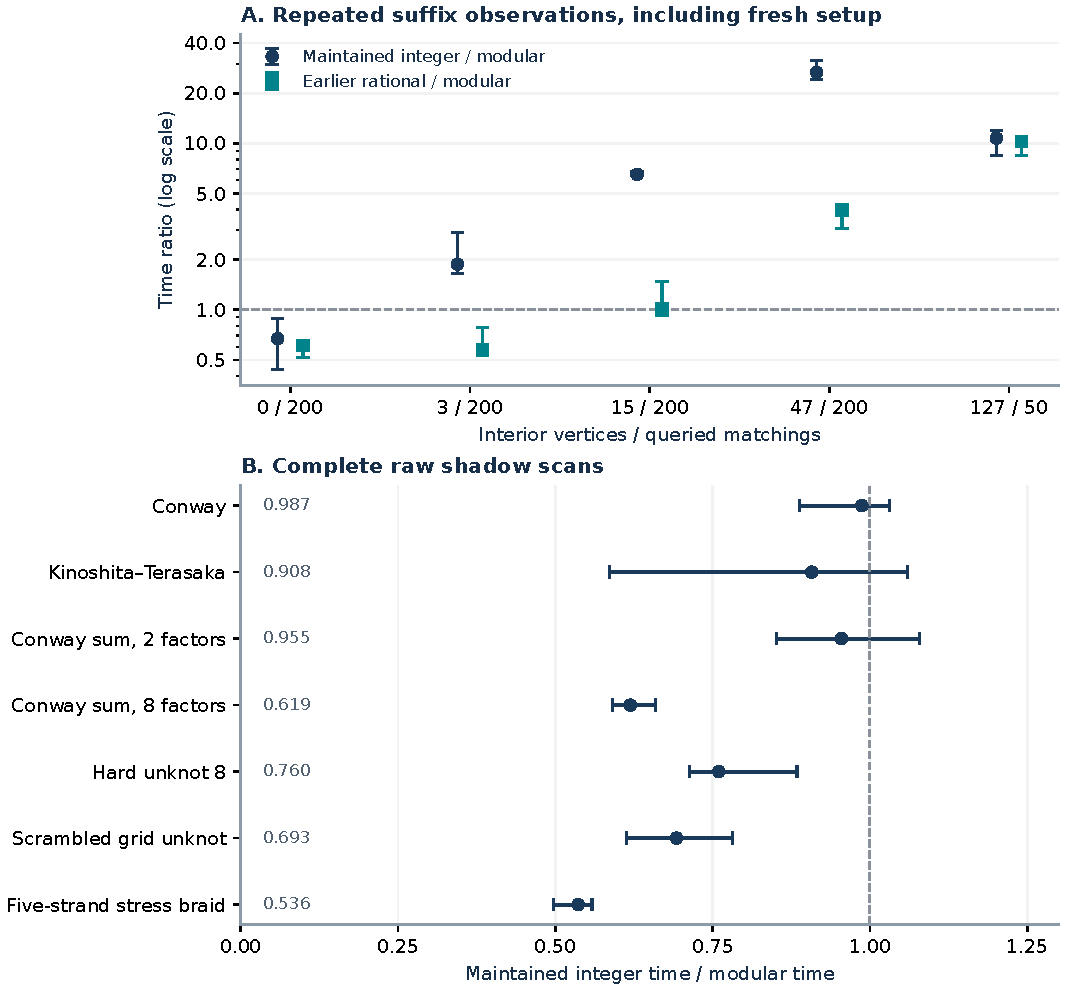
\includegraphics[width=0.99\textwidth]{figures/performance.pdf}
\caption{Measured gains depend strongly on scope. A ratio above one favors the
modular implementation. Points show medians of five paired ratios; whiskers
show the observed range. Panel A includes fresh geometry and response setup.
Panel B measures complete raw scans, where all seven median ratios are below
one. The two panels use different axis scales.}
\label{fig:performance}
\end{figure}

\subsection{The full scans are slower on this corpus}

\begin{table}[htbp]
\centering\small
\caption{The raw scans do not show an overall recognition gain.}
\label{tab:recognition}
\begin{tabular}{@{}lrrrr@{}}
\toprule
Input & Integer (ms) & Modular (ms) & Raw ratio & Filters off\\
\midrule
Conway & 4.774 & 4.895 & 0.987 & 0.969\\
Kinoshita--Terasaka & 5.396 & 5.737 & 0.908 & 0.873\\
Conway sum, 2 factors & 8.807 & 9.494 & 0.955 & 0.961\\
Conway sum, 8 factors & 10.113 & 16.186 & 0.619 & 0.635\\
Hard unknot 8 & 0.972 & 1.264 & 0.760 & 0.803\\
Scrambled grid unknot & 0.513 & 0.741 & 0.693 & 0.677\\
Five-strand stress braid & 1.186 & 2.158 & 0.536 & 0.515\\
\bottomrule
\end{tabular}
\par\smallskip\begin{minipage}{0.97\textwidth}\footnotesize
The first two columns time raw shadow scans. Raw ratio is the paired integer/modular ratio in that scope. Filters off is the corresponding ratio through the public recognition pipeline with its earlier filters disabled. All seven ordinary default-filter runs stop before either shadow backend.
\end{minipage}
\end{table}


The seven examples cover the Conway knot, the Kinoshita--Terasaka knot, visible
connected sums of the Conway knot, two unknot examples, and a five-strand stress
braid. The example names identify the saved input files or generators in the
package; they are not a random sample of knots at those crossing numbers.

Every raw-scan median ratio is below one. The observed range is 0.536--0.987,
with the largest relative regression on the short stress-braid scan. Calling
through the public recognition pipeline with its preceding filters disabled
gives the same qualitative result, with median ratios 0.515--0.969. These
absolute runtimes are short, but the experiment provides no evidence that the
modular backend improves complete scans on this corpus.

The normal pipeline is a separate and especially important control. All seven
examples are decided before either shadow observer is invoked: Conway and
Kinoshita--Terasaka by the modular Jones filter; their visible sums by
factorization followed by that filter; the hard-unknot example by the
three-braid free-product route; the scrambled grid unknot by Reidemeister
reduction; and the stress braid by the modular Alexander filter. Near-one
ratios in those runs measure front-end timing variation. They must not be
reported as evidence for the new continuation.

Across all warm-ups and samples, 24,200 repeated vector comparisons and 2,013
repeated status comparisons agree. These are validation-event counts,
\emph{not} counts of distinct diagrams or completions. Completed integer and
rational vectors agree with the new vectors modulo 65521. Status equality is
required; equality of every stopping stage or intermediate method is not.
The hashed observer sources did not change during the benchmark.

\subsection{The supported performance conclusion}

Boundary reuse removes repeated dependence on a large suffix interior, and
finite-field arithmetic can improve substantially on the rational response
when that interior is large. The production measurements justify keeping this
capability available. The complete-scan results simultaneously show that eager
preparation is not a successful universal policy. A scheduler must estimate
whether a suffix will receive enough distinct useful queries before the scan
moves on or another obstruction succeeds.

The next benchmark should hold out a corpus where the earlier structural,
Alexander, and Jones filters genuinely remain inconclusive, include large
interior graphs with few queries, and measure successful early stops and total
scan work. A claimed default-policy improvement should survive that test with
setup, failed probes, prime refinement, cache memory, and timeouts all charged.

\section{Further research questions and proposed priorities}
\label{sec:research}

The arithmetic improvement is useful enough to integrate as an optional
capability. The evidence suggests a different order of priorities for obtaining
practical speed-ups and for proving a quasi-polynomial theorem. The former
needs better scheduling and reuse; the latter needs a representation theorem
and a bound on decisive work. The following questions state both the proposed
work and the evidence that would count as progress.

\subsection{Near-term implementation and experimental questions}

\paragraph{Q1. When should a suffix pay for a response?}
Can a scheduler predict the number of distinct useful matching and partition
queries before the suffix changes? A candidate decision rule should compare
measured direct-query cost with preparation cost plus expected boundary-query
cost, using $v-t$, $t$, projected query count, and the number of likely prime
passes. It should also account for the chance that the exact Euler prefilter
or first few direct queries stop the scan. A concrete milestone is an opt-in
hybrid that selects direct integer, rational response, or modular response
on a held-out corpus and improves total recognition time with every failed
probe charged. The current seven raw regressions make this the first
performance priority. A model fitted only to the favorable pure-tail stream
would not be adequate evidence.

\paragraph{Q2. Can a response survive a change of suffix?}
Removing one crossing changes both edges and the cut-face fragmentation. It can
split a region, create new terminals, and change the radical dimension. A
correct incremental update therefore needs a precise map between successive
vertex spaces, not just a rank-one edge update to a fixed Laplacian. Develop
an update calculus for fragment splits, terminal promotions, and edge deletion,
with a rebuild path when the pivot profile changes. The useful theorem would
bound amortized update work in terms of the changed frontier neighborhood.
The useful experiment would include many consecutive observed stages with
few queries per stage, where full rebuilding currently loses.

\paragraph{Q3. How should articulation blocks and sparse elimination combine?}
The maintained direct observer already factors at articulation points. A
boundary response could eliminate terminal-free blocks separately and retain
small interfaces at blocks that contain frontier terminals. The challenge is
to prove the gluing formula with signed weights, zero tree factors, and singular
interiors; a division by an apparently harmless block determinant can fail
modulo a prime. Establish a singular-safe block response and compare it with
both existing articulation factoring and dense modular preparation. Measure
fill-in, temporary memory, and cost at exceptional primes, as well as elapsed
time on nonsingular examples.

\paragraph{Q4. Which certified coefficient bounds repay their cost?}
The bound $C_a\le s_a2^{n-1}$ is universal but can be loose. Candidate refinements
include the unsigned spanning-tree count of the actual graph, products of
blockwise bounds, bridge reductions, and degree-based determinant bounds. A
bound should be computed once and reused across completions when possible;
otherwise its cost can exceed the modular observation it was meant to save.
The target is a proved $C_a'$ together with a measured reduction in prime passes
or exact-threshold completion time. Signed cancellation may improve the actual
coefficient, but cannot justify shrinking a certified bound without evidence.

\paragraph{Q5. Can prime scheduling exploit the exposure theorem?}
\Cref{prop:prime-exposure} bounds how many primes can hide an existing
obstruction. Use it to design a policy choosing between one more independent
prime, another CRT pass, and continuing the scan. An asymptotic version should
supply enough primes automatically and charge their generation and validation.
A practical version should distinguish a large default prime from a random
prime-pool experiment, retain monotone CRT information, and report the cost
of inconclusive passes. Prime choice must never change the meaning of a
positive result. The 70 misses at prime three are a useful adversarial check,
not a reason to label the method probabilistic or unsound.

\paragraph{Q6. What is the true memory cost of continuation reuse?}
Only the active residual matrices are boundary-sized. Completed-value keys and
records can accumulate across stages, and algebraic generator storage may
dominate everything. Introduce a memory ledger for geometry, prime responses,
partition caches, matching keys, exact Euler integers, and scanner objects.
Study bounded caches or stage-local eviction with reconstruction charged.
A credible performance report should include peak memory and the number of
retained objects, not only the largest query matrix. This may reveal a regime
where recomputation is preferable to retaining all exact completion values.

\subsection{Questions that address the quasi-polynomial barrier}

\paragraph{Q7. Which continuation behaviors admit a succinct quotient?}
Equality of boundary matchings is too coarse to identify chain complexes with
different differentials. Seek an equivalence relation on relative complexes
that preserves the needed threshold decision under all admissible future
crossings or actual suffixes, and that is stable under tensoring, delooping,
and cancellation. The essential result would bound the number and bit size of
its states by $2^{(\log N)^{O(1)}}$ and give constructive transition rules.
A finite table of scalar Euler observations alone is unlikely to determine
all future homological behavior; this should be tested with counterexamples
before adopting it as a state representation. Any successful quotient must
retain enough information to justify the marked homotopies, not merely $d^2=0$.

\paragraph{Q8. Is there a family theorem for the first decisive observation?}
For a specified diagram family and order policy, can one bound the number of
represented objects and stages before $B_4>1$, or before a rank-two contraction
is exhibited? The arithmetic completion theorem starts only after an exact
obstruction is present. It says nothing about when that happens. A useful
intermediate target is an explicit family beyond the already solved structural
cases, with a proved stopping-stage bound and a certified complexity expression
in its parameters. Failed examples should retain the exact sequence of prefix
bounds, so a proposed detection lemma can be falsified by genuine complexes.

\paragraph{Q9. Can larger residue systems remain efficiently observable?}
Residues modulo eight or higher powers of two refine quantum grading and can
retain cancellations lost modulo four. Investigate whether their evaluations
admit a manageable transfer representation on bounded interfaces. The special
value at $i$ has a spanning-tree determinant formula; higher roots do not
inherit that formula automatically. A successful extension needs three proofs:
that the residue norm still bounds completed homology, that the relevant
integer or cyclotomic data are computed exactly, and that their observation
cost has the claimed dependence on boundary width. A larger invariant that
requires exponential work in the suffix would not resolve the present barrier.

\paragraph{Q10. Can homological information be compressed without changing fields?}
The auxiliary primes in this paper reduce integer Euler data. They cannot be
used to compute a generic odd-characteristic Khovanov rank and silently treat
it as the rank over $\F_2$. Investigate compact descriptions of persistent
cancellations, module decompositions, or continuation-compatible rank defects
\emph{over the actual coefficient field}. The maintained interval and scalar-
splitting backends provide concrete comparison points. A new theorem should
state exactly which operations preserve the compressed description and what
happens when that description must expand. The three-braid structural formulas
suggest that family-specific symbolic answers can be much smaller than
explicit bases \cite{kelomaki}.

\paragraph{Q11. What geometric decomposition gives the right width measure?}
A polylogarithmic number of frontier darts would bound the oracle table, but
it is not guaranteed by the current crossing-order search. Investigate
hierarchical decompositions whose interfaces carry both the tangle data and
sufficient algebraic summaries. A useful theorem must control interface size,
number of pieces, transition cost, and the growth of multiplicities and
coefficient descriptions simultaneously. If only a planar separator estimate
with a much larger boundary is available, state the resulting subexponential
bound honestly; it does not become quasi-polynomial through terminology.
Connections to hierarchy-based topological methods are promising only after
the translation cost is made explicit.

\paragraph{Q12. Can independently verified compressed contractions replace replay?}
The current verifier reconstructs the entire prefix. A more useful certificate
would encode contractions and direct-sum decompositions in a form whose local
identities can be checked without expanding every intermediate complex. Study
straight-line descriptions of maps and homotopies, canonical sharing, and
certified transfer across a decomposition tree. The certificate must include
its own size bound and account for zero tests and equality of compressed maps.
A short list of moves is insufficient if one move refers to an exponentially
large object. A constructive bound here would address both practical replay
cost and a major part of \cref{prop:conditional}.

\subsection{External algorithm audits and integration milestones}

Two literature tracks deserve separate, explicit audits. Lackenby's hierarchy
program supplies a geometric framework and efficiently checkable objects;
an implementation study should identify which construction and encoding bounds
are already proved and which speed-up lemmas remain proposed
\cite{lackenby2026,lackenbytalk}. Musick's September 2026 polynomial-time claim
should be assessed independently: formalize its state representation, verify
that every claimed local move is discoverable within the compressed encoding,
and prove a bound on the total descriptions created, including overwritten
or retained grammar versions \cite{musick}. This article neither adopts that
claim nor supplies a counterexample. Its relevance is that a serious current
research program should investigate a directly competing claimed algorithm
instead of declaring it absent.

For ProveIt, the immediate integration sequence is concrete. Add the optional
backend and its replay tests against the pinned source. Preserve the recorded
arithmetic and actual-diagram audits. Keep the raw timing samples and the
negative complete-scan results next to the favorable response experiment.
Then evaluate a scheduling change as a separate patch with a new held-out
corpus. The inherited normal-surface I/O defect should also receive a separate
focused repair rather than an unexplained test exclusion.

The next mathematical milestone should be a family theorem controlling the
size of a continuation-compatible representation through a decisive event.
The modular response provides a proved inexpensive observation interface to
attach to that theorem. Establishing the representation and stopping bounds
is the work that would turn the present performance improvement into progress
on a general quasi-polynomial recognition guarantee.

% Bibliographic metadata checked against primary author, publisher, and arXiv
% records on 8 October 2026.  Citation keys match the article draft.
% The extra entry lackenbyabstract supports the stronger exponent appearing in
% the Oxford seminar announcement; it is distinct from the technical handout.
\begin{thebibliography}{99}

\bibitem{barnatan2005}
Dror Bar-Natan,
\emph{Khovanov's homology for tangles and cobordisms},
Geometry \& Topology \textbf{9} (2005), 1443--1499.
\href{https://doi.org/10.2140/gt.2005.9.1443}{doi:10.2140/gt.2005.9.1443}.
\url{https://arxiv.org/abs/math/0410495}.

\bibitem{barnatan2007}
Dror Bar-Natan,
\emph{Fast Khovanov homology computations},
Journal of Knot Theory and Its Ramifications \textbf{16} (2007), no.~3,
243--255.
\url{https://arxiv.org/abs/math/0606318}.
Author's publication record:
\url{https://www.math.toronto.edu/~drorbn/papers/FastKh/}.

\bibitem{kronheim}
P.~B. Kronheimer and T.~S. Mrowka,
\emph{Khovanov homology is an unknot-detector},
Publications Math\'ematiques de l'IH\'ES \textbf{113} (2011), 97--208.
\href{https://doi.org/10.1007/s10240-010-0030-y}{doi:10.1007/s10240-010-0030-y}.
\url{https://arxiv.org/abs/1005.4346}.

\bibitem{kenyonwilson}
Richard W. Kenyon and David B. Wilson,
\emph{Boundary partitions in trees and dimers},
Transactions of the American Mathematical Society \textbf{363} (2011),
1325--1364.
\href{https://doi.org/10.1090/S0002-9947-2010-04964-5}{doi:10.1090/S0002-9947-2010-04964-5}.
\url{https://arxiv.org/abs/math/0608422}.

\bibitem{dumasurbanska}
Jean-Guillaume Dumas and Anna Urba\'nska,
\emph{An introspective algorithm for the integer determinant},
expanded research paper, arXiv:cs/0511066v5, 13 September 2007.
Preliminary version presented at \emph{Transgressive Computing 2006},
Granada, 2006.
\url{https://arxiv.org/abs/cs/0511066v5}.

\bibitem{kelomaki}
Tuomas Kelom\"aki and Dirk Sch\"utz,
\emph{On computational complexity of Khovanov homology},
preprint, arXiv:2601.02119v1, 5 January 2026.
\url{https://arxiv.org/abs/2601.02119v1}.

\bibitem{lackenby2026}
Marc Lackenby,
\emph{Incompressible surfaces, hierarchies and unknot recognition},
preprint, arXiv:2607.23350v1, 25 July 2026.
\url{https://arxiv.org/abs/2607.23350v1}.

\bibitem{lackenbytalk}
Marc Lackenby,
\emph{Unknot recognition in quasi-polynomial time},
Oxford topology seminar technical handout, March 2021, 34 pages.
\url{https://people.maths.ox.ac.uk/lackenby/quasipolynomial-talk-oxford-compressed.pdf}.

\bibitem{lackenbyabstract}
Marc Lackenby,
\emph{Unknot recognition in quasi-polynomial time},
Oxford Mathematical Institute topology seminar announcement and abstract,
15 March 2021.
\url{https://www.maths.ox.ac.uk/node/60914}.

\bibitem{musick}
Chad Musick,
\emph{Locally minimal bridge presentations of knots},
preprint, arXiv:2609.06492v2, 20 September 2026.
\url{https://arxiv.org/abs/2609.06492v2}.

\bibitem{proveit}
Vladimir Reshetnikov,
\emph{ProveIt: Topology/UnknotRecognition},
source code and research reports, pinned revision
\texttt{8a95834940cf77cdab1b39571ffc102ca8b6bede}.
\url{https://github.com/VladimirReshetnikov/ProveIt/tree/8a95834940cf77cdab1b39571ffc102ca8b6bede/Topology/UnknotRecognition}.
Source audit dated 8 October 2026.

\bibitem{chebyshevnotes}
J.~Barkley Rosser and Lowell Schoenfeld,
\emph{Approximate formulas for some functions of prime numbers},
Illinois Journal of Mathematics \textbf{6} (1962), no.~1, 64--94, Theorem 4.
\href{https://doi.org/10.1215/ijm/1255631807}{doi:10.1215/ijm/1255631807}.
Original-paper PDF mirror:
\url{https://denisevellachemla.eu/Rosser-Schoenfeld-1962.pdf}.

\end{thebibliography}

\end{document}
